\section{Registers}
\label{sec:registers}

\begin{itemize}[leftmargin=0.7cm]
  \item A \textbf{register} is a \textit{group of flip-flops}, each one of which shares a common clock and is capable of storing one bit of information. An $n$-bit register consists of a group of $n$ flip-flops capable of storing $n$ bits of binary information. In addition to the flip-flops, a register may have combinational gates that perform certain data-processing tasks. 

  In its broadest definition, a register consists of a group of flip-flops together with gates that affect their operation. The flip-flops hold the binary information, and the gates determine how the information is transferred into the register.

  \item A \textbf{counter} is essentially \textit{a register that goes through a predetermined sequence of binary states}. The gates in the counter are connected in such a way as to produce the prescribed sequence of states. Although counters are a special type of register, it is common to differentiate them by giving them a different name.
\end{itemize}

\noindent The simplest register is one that consists of only flip-flops, without any gates. Figure 1 shows such a register constructed with four $D$-type flip-flops to form a four-bit data storage register.


\subsection{Register with Parallel Load}
\label{subsec:register-with-parallel-load}

The transfer of new information into a register is referred to as \textit{loading} or \textit{updating} the register. If all the bits of the register are loaded simultaneously with a common clock pulse, we say that the loading is done in \textit{parallel}.

If the contents of the register must be left unchanged, the inputs must be held constant or the clock must be inhibited from the circuit.
\begin{itemize}[leftmargin=0.7cm]
  \item In the first case, the data bus driving the register would be unavailable for other traffic.
  \item In the second case, the clock can be inhibited from reaching the register by controlling the clock input signal with an enabling gate.
\end{itemize}

The solution can be implementing the additional gates in either the data bus or the output of the register to allow data to load or update. In Fig. 2, load input is implemented.

\vspace*{\fill}
\columnbreak

\begin{figure}[H]
  \centering
  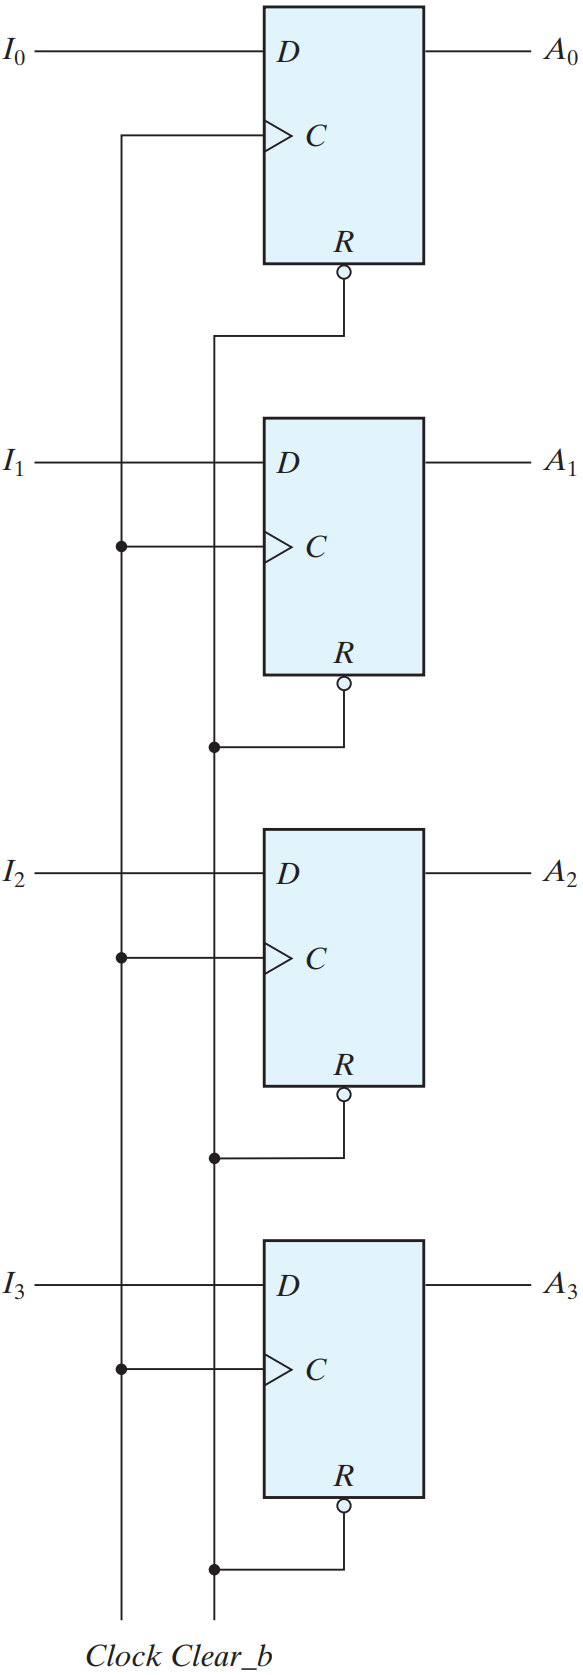
\includegraphics[width=.9\linewidth]{img/fig-6.1.png}
  \caption{Four-bit register}
  \label{fig:6.1}
\end{figure}

\begin{figure}[H]
  \centering
  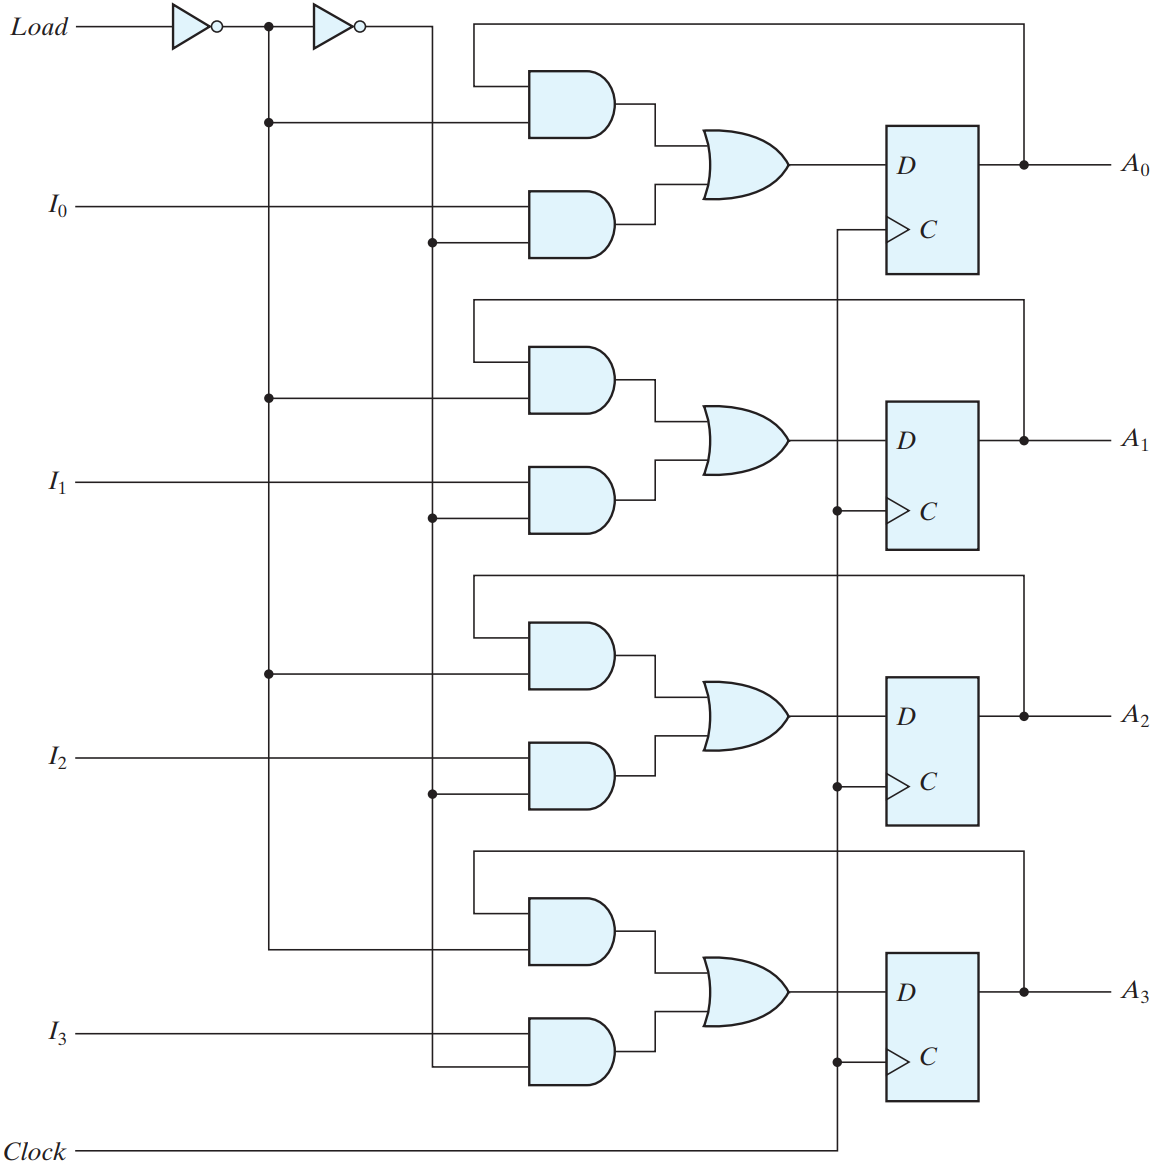
\includegraphics[width=\linewidth]{img/fig-6.2.png}
  \caption{Four-bit register with parallel load}
  \label{fig:6.2}
\end{figure}
